\documentclass[hyperref, notheorems]{beamer}

% PACKAGES
\usepackage[utf8]{inputenc}
\usepackage{geometry}
\usepackage{appendix}
\usepackage{ytableau}
\usepackage{hyperref}
\usepackage{amsmath}
\usepackage{soul}
\usepackage{amssymb}
\usepackage{amsthm}
\usepackage{mathrsfs}
\usepackage{tcolorbox}
\usepackage{pgf}
\usepackage{tikz}
\usepackage{tikz-cd}
\usetikzlibrary{arrows,decorations.markings}
\usepackage{pst-platon}
\usepackage{transparent}
\usepackage{graphicx}
\usepackage{xcolor}

% NEW ENVIRONMENTS
\newenvironment{reference}{\begin{tcolorbox}[width=\linewidth,baseline=\tcbtextheight+\baselineskip]}{\end{tcolorbox}}
\newenvironment{creference}{\begin{tcolorbox}[width=\linewidth,baseline=\tcbtextheight+\baselineskip]\centering}{\end{tcolorbox}}

% NEW AND REDEFINED COMMANDS
\newcommand{\legendre}[2]{\genfrac{(}{)}{0.5pt}{0}{#1}{#2}}
\newcommand{\tmod}[1]{\text{ mod }#1}
\newcommand{\xto}[1]{\xrightarrow{#1}}
\newcommand{\xfrom}[1]{\xleftarrow{#1}}
\newcommand{\normal}{\mathrel{\unlhd}}
\newcommand{\mf}[1]{\mathfrak{#1}}
\newcommand{\Mat}{\mathrm{Mat}}
\newcommand{\GL}{\mathrm{GL}}
\newcommand{\SL}{\mathrm{SL}}
\renewcommand{\O}{\mathrm{O}}
\newcommand{\N}{\mathbb{N}}
\newcommand{\Z}{\mathbb{Z}}
\newcommand{\Q}{\mathbb{Q}}
\newcommand{\R}{\mathbb{R}}
\newcommand{\C}{\mathbb{C}}
\newcommand{\F}{\mathbb{F}}
\renewcommand{\H}{\mathbb{H}}
\renewcommand{\P}{\mathbb{P}}
\renewcommand{\a}{\alpha}
\renewcommand{\b}{\beta}
\newcommand{\g}{\gamma}
\renewcommand{\d}{\delta}
\newcommand{\e}{\epsilon}
\newcommand{\z}{\zeta}
\renewcommand{\t}{\theta}
\renewcommand{\i}{\iota}
\renewcommand{\k}{\kappa}
\renewcommand{\l}{\lambda}
\newcommand{\s}{\sigma}
\renewcommand{\o}{\omega}
\newcommand{\vphi}{\varphi}
\newcommand{\emt}{\varnothing}
\newcommand{\x}{\times}
\newcommand{\ox}{\otimes}
\newcommand{\op}{\oplus}
\newcommand{\del}{\partial}
\DeclareMathOperator{\id}{\textrm{id}}
\DeclareMathOperator{\sgn}{\mathrm{sgn}}
\DeclareMathOperator{\im}{\mathrm{im}}
\DeclareMathOperator{\rk}{\mathrm{rk}}
\DeclareMathOperator{\tr}{\mathrm{trace}}
\DeclareMathOperator{\ord}{\mathrm{ord}}
\DeclareMathOperator{\Hom}{\mathrm{Hom}}
\DeclareMathOperator{\End}{\mathrm{End}}
\DeclareMathOperator{\Aut}{\mathrm{Aut}}
\DeclareMathOperator{\Tor}{\mathrm{Tor}}
\DeclareMathOperator{\Ann}{\mathrm{Ann}}
\DeclareMathOperator{\Gal}{\mathrm{Gal}}
\DeclareMathOperator{\spn}{\mathrm{span}}
\DeclareMathOperator{\diam}{\mathrm{diam}}
\DeclareMathOperator{\Real}{\mathrm{Real}}
\DeclareMathOperator{\Imag}{\mathrm{Imag}}
\DeclareMathOperator{\Trace}{\mathrm{Trace}}
\DeclareMathOperator{\Norm}{\mathrm{Norm}}
\usepackage{quiver}
\newcommand{\afrak}{\mathfrak{a}}
\newcommand{\Rbb}{\mathbb{R}}
\newcommand{\Zbb}{\mathbb{Z}}
\newcommand{\Pbb}{\mathbb{P}}
\newcommand{\Qbb}{\mathbb{Q}}
\newcommand{\Cbb}{\mathbb{C}}
\newcommand{\Abb}{\mathbb{A}}
\newcommand{\Vbb}{\mathbb{V}}
\newcommand{\txtblue}{\textcolor{blue}}
\newcommand{\Ydd}{Y_{\Tilde{\Delta} /\Delta}}
\newcommand{\Wdd}{W_{\Tilde{\Delta} /\Delta}}
\usepackage{mathtools}
% BACK OF POCKET TOOLS
% [label=(\roman*)]
% [label=(\alph*)]
% [label=(\arabic{enumi})]


% SPECIAL COMMANDS
\newcommand{\smathcal}[1]{
    \mathchoice
    {{\scriptstyle\mathcal{#1}}}
    {{\scriptstyle\mathcal{#1}}}
    {{\scriptscriptstyle\mathcal{#1}}}
    {\scalebox{.7}{$\scriptscriptstyle\mathcal{#1}$}}
}

% TIKZ PREAMBLE
\newcommand{\disc}{\draw(0,0) [fill=gray] circle (1cm);}
\newcommand{\strip}[1]{
\fill [white,even odd rule,rotate=#1] (1,0) circle[radius=0.42cm] circle[radius=0.28cm];
\fill [lightgray,even odd rule,rotate=#1] (1,0) circle[radius=0.4cm] circle[radius=0.3cm];}
\newcommand{\varstrip}[3]{
\fill [white,even odd rule,rotate=#1] (1,0) circle[radius=0.3*#2+0.12*#3] circle[radius=0.3*#2-0.02*#3];
\fill [lightgray,even odd rule,rotate=#1] (1,0) circle[radius=0.3*#2+0.1*#3] circle[radius=0.3*#2];}
\newcommand{\mstrip}[1]{
\fill [white,rotate=#1] (0.8,0.38) -- (1.25, 0.23) -- (1.43,0.1) -- (1.43,-0.1) -- (1.25,-0.23) -- (0.8,-0.38) -- (0.8,-0.22) -- (1,-0.17) -- (1.3,-0.05) -- (1.3,0.05) -- (0.8,0.22) -- (1,0.17) -- cycle;
\draw [thick,domain=-0.4:0.4,rotate=#1+2.5] plot ({1.4-7*\x*\x}, {\x});
\fill [white,rotate=#1] (1.36,0.01) circle(0.04);
\draw [thick,domain=-0.4:0.4,rotate=#1-2.5] plot ({1.4-7*\x*\x}, {\x});
}
\tikzset{vertex/.style = {shape=circle,draw,minimum size=1.5em}}
\tikzset{edge/.style = {->,> = latex'}}
\tikzset{->-/.style={decoration={
  markings,
  mark=at position 0.55 with {\arrow{stealth}}},postaction={decorate}}}

%BEAMER PREAMBLE
\usefonttheme[onlymath]{serif}
\definecolor{burgundy}{rgb}{0.5, 0.0, 0.13}
\usetheme[sidebarleft]{Caltech}
\setbeamertemplate{footline}[frame number]
\setbeamercovered{transparent}
\theoremstyle{definition}
\newtheorem{definition}{\translate{Definition}}
\newtheorem{theorem}{\translate{Theorem}}
\newtheorem{example}{\translate{Example}}
\newtheorem{conjecture}{\translate{Conjecture}}
% TITLE
\title{Wavelets in $p$-adic Analysis}
\author{Mattie Ji}
\institute{APMA 1940Y - Wavelets and Applications}
\date{May 3rd, 2023}
\AtBeginSection[]{
  \begin{frame}
    \frametitle{Outline}
    \tableofcontents[currentsection]
  \end{frame}
}

\usepackage{bibentry}
\nobibliography*  

%Table of Content

\begin{document}

\begin{frame}
    \titlepage
\end{frame}

% \begin{frame}
%     \frametitle{Outline}
%     \tableofcontents
% \end{frame}

% Hide subsections from table of contents
% \begin{frame}{Outline}
%     \tableofcontents[hideallsubsections]
% \end{frame}
% https://latex-beamer.com/tutorials/table-of-contents/

% Presentation structure
\begin{frame}{Motivation:}
In class, given a scaling function $\varphi$ and its associated wavelet $\psi$, we constructed the incremental spaces $W_j$ as
\[W_j = \spn \{\psi(\txtblue{2^j} t - k)\ :\ k \in \Zbb\}\]

\begin{block}{Question:}
    What if we replace $2$ with a prime number $p$?
\end{block}

This observation is intricately related to a number system called the ``\txtblue{$p$-adic numbers}".
\end{frame}



\begin{frame}{The $p$-adic norm}
Let $p$ be a prime number,
\begin{itemize}
    \item For any non-zero $x \in \Qbb$, $x$ may be written as
    \[x = p^n \frac{a}{b},\quad \text{$a$ and $b$ are coprime to $p$}\]
    We define the \txtblue{$p$-adic norm} $|\bullet|_p: \Qbb \to \Rbb$ as
    \[|x|_p = \begin{cases}
    p^{-n}, \text{ if $x = p^n \frac{a}{b}$}\\
    0, \text{ if $x = 0$}
    \end{cases}\]
    \item For example, when $p = 2$,
    \[|3 - 1|_2 = \frac{1}{2} \text{ and } |1025 - 1|_2 = \frac{1}{2^{10}}\]
    \item In the $2$-adic norm, $1$ and $3$ are very far away, but $1$ and $1025$ are really close.
\end{itemize}
\end{frame}

\begin{frame}{The $p$-adic numbers}
We define the \txtblue{$p$-adic numbers $\Qbb_p$} as the \txtblue{metric completion} of $\Qbb$ with respect to $|\bullet|_p$. $\Qbb_p$ also extends $\Qbb$ as a field.\\
\vspace{\baselineskip}
Although $\Rbb$ and $\Qbb_p$ are both constructed from $\Qbb$, they are very different! For example,
\begin{itemize}
    \item Every point in $\Qbb_p$ is disconnected from one another.
    \item The integers are actually bounded in $\Qbb_p$.
\end{itemize}
    % \item Concretely, every non-zero element $x \in \Qbb_p$ may be represented uniquely as a \txtblue{``Laurent series"} of the form
    % \[x = \sum_{i = k}^{\infty} a_i p^i,\quad a_i = 0, ..., p-1, k \in \Zbb\]
    % whose addition and multiplication operations respect the series expression here.
    % \item The $p$-adic norm of $x$ may be computed as
    % \[|x|_p = p^{-v_p(x)}\]
    % where $v_p(x)$ (the \txtblue{$p$-adic valuation}) is the exponent of $p$ in the first non-zero term of the series representation.
\end{frame}

\begin{frame}{Why $p$-adic analysis?}

\txtblue{Q: Why should we care about $p$-adic analysis?}\\
\vspace{\baselineskip}

All experimental and observational data we collect are actually rational numbers. Sometimes $\Qbb_p$ may be an appropriate extension than $\Rbb$!
\begin{itemize}
    \item In particle physics, there's a fundamental restriction on how small we can measure an object. This is known as the \txtblue{Planck Length}.\\
    \vspace{\baselineskip}
    This discrete nature suggests that $\Qbb_p$ may be more intuitive as a geometrical interpretation of space-time (see \cite{volovich_1987})

    \item Besides physics, $p$-adic analysis has found applications in Biological Systems, Stochastic Processes, Data Mining, and more. (see \cite{dragovich_khrennikov_kozyrev_volovich_zelenov_2017})
\end{itemize}
\end{frame}

\begin{frame}{Where do Wavelets come in?}

\begin{itemize}
    
    \item In $p$-adic analysis, the analog of real fractional differentiations is defined using what's called a ``\txtblue{Vladimirov operator}" (\cite{vladimirov_1988}):
    \item For $f \in L^2(\Qbb_p)$ and $\alpha > 0$
        \[D^\alpha f(x) = \frac{p^\alpha - 1}{1 - p^{-1 - \alpha}} \int_{\Qbb_p} \frac{f(x) - f(y)}{|x - y|^{1+\alpha}_p} d\mu(y)\]
    \item Wouldn't it be great if we can diagonalize this operator?
\end{itemize}
\end{frame}

\begin{frame}{Where do Wavelets come in?}
\begin{itemize}
    \item In $2002$, Kozyrev pioneered the field of $p$-adic wavelets by showing that there's a correspondence with \txtblue{the Haar Wavelet decomposition of $L^2(\Rbb_+)$} and \txtblue{eigenvectors of the Vladimirov operator in $L^2(\Qbb_p)$} \cite{kozyrev_2002}.
    \item Hence, the theory of wavelets can be readily applied to $p$-adic fractional differentiations.
    \item We will spend the rest of this presentation discussing this result.
\end{itemize}
\end{frame}

% \begin{frame}{Integration on the $p$-adic numbers}

% \txtblue{Q: What do we mean by $L^2(\Qbb_p)$?}\\
% \vspace{\baselineskip}

% \begin{itemize}
%     \item Given $f: \Qbb_p \to \Cbb$, the integration of $f$ on $\Qbb_p$ can be done with respect to the \txtblue{normalized Haar measure $\mu$} on $\Qbb_p$.
%     \item Concretely, for any $x \in \Qbb_p$, we define $B_r(x)$ as the set $\{y \in \Qbb_p\ |\ |x - y|_p < r\}$, then $\mu$ is given in the natural way as:
%     \[\mu(B_r(x)) = \diam B_r(x)\]
%     \item Intuitively, one may think of $\mu$ as the ``\txtblue{Lebesgue measure}" of $\Qbb_p$.
%     \item $L^2(\Qbb_p)$ then refers to the functions $f:\Qbb_p \to \Cbb$ such that
%     \[\int_{\Qbb_p} f \overline{f} d\mu < \infty\]
% \end{itemize}
% \end{frame}

\begin{frame}{Extending Haar Wavelets\footnote{The rest of the slides are all based on Kozyrev's original paper.}}
    In class, the Haar Wavelet $\psi^H$ is given as the difference of two characteristic functions:
    \[\psi^H(x) = \chi_{[0, \frac{1}{2})}(x) - \chi_{[\frac{1}{2}, 1]}(x)\]
    The construction here uses \txtblue{$2$ characteristic functions}, and when we extended this into a decomposition of $L^2(\Rbb_+)$, we were considering \txtblue{multiplications by $2$}.
    \vspace{\baselineskip}\\
    It turns out that the original Haar Wavelet is really good at interpreting the \txtblue{Vladimirov operator} in $\Qbb_2$, but for $\Qbb_p$ in general, we wish to extend this a ``\txtblue{$p$-Haar wavelet}".
\end{frame}

\begin{frame}{Extending Haar Wavelets}
    We define the \txtblue{$p$-Haar wavelet basis} of $L^2(\Rbb_+)$ as follows:
    \begin{itemize}
        \item For $1 \leq k \leq p - 1$, the $p$-Haar wavelet function $\psi_k^{(p)}(x)$ is given as
        \[\psi_k^{(p)}(x) = \sum_{\ell = 0}^{p-1} e^{\frac{2\pi i k \ell}{p}} \chi_{[\frac{\ell}{p}, \frac{\ell + 1}{p}]}(x)\]
        \item Consider the incremental spaces $W_j$ given by
        \[W_j = \spn\{\psi_k^{(p)}(p^{-j} x - n) : n \in \Zbb_+, k = 1, ..., p-1  \}\]
        Then we in fact have that
        \[\overline{\bigoplus_{j \in \Zbb} W_j} = L^2(\Rbb_+)\]
    \end{itemize}
\ul{When $p = 2$, this is exactly the Haar wavelet decomposition.}  
\end{frame}

\begin{frame}{Example: $p = 3$}

For $k = 1$, we obtain the following graphs of $\psi_1^{(3)}(x)$:

\begin{figure}[!tbp]
  \centering
  \begin{minipage}[b]{0.45\textwidth}
    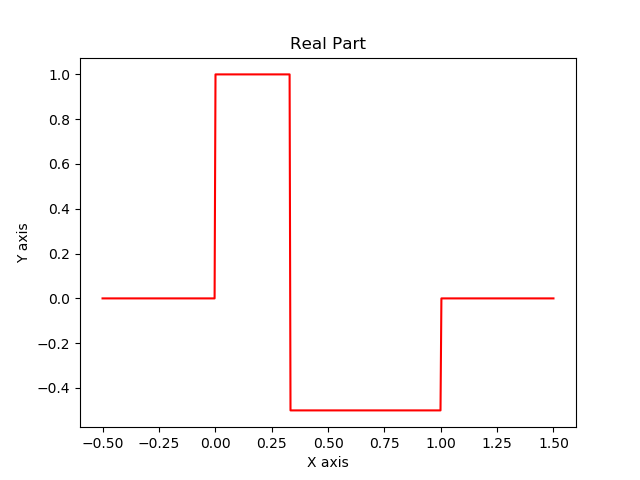
\includegraphics[width=\textwidth]{graphics/real_1.png}
    \caption{$\Real(\psi^{(3)}_1)$}
  \end{minipage}
  \hfill
  \begin{minipage}[b]{0.45\textwidth}
    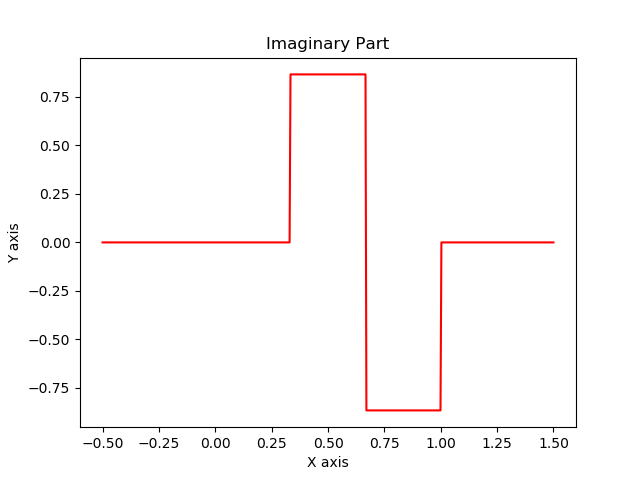
\includegraphics[width=\textwidth]{graphics/imag_1.png}
    \caption{$\Imag(\psi^{(3)}_1)$}
  \end{minipage}
\end{figure}
\end{frame}

\begin{frame}{Example: $p = 3$}

For $k = 2$, we obtain the following graphs of $\psi_2^{(3)}(x)$:

\begin{figure}[!tbp]
  \centering
  \begin{minipage}[b]{0.45\textwidth}
    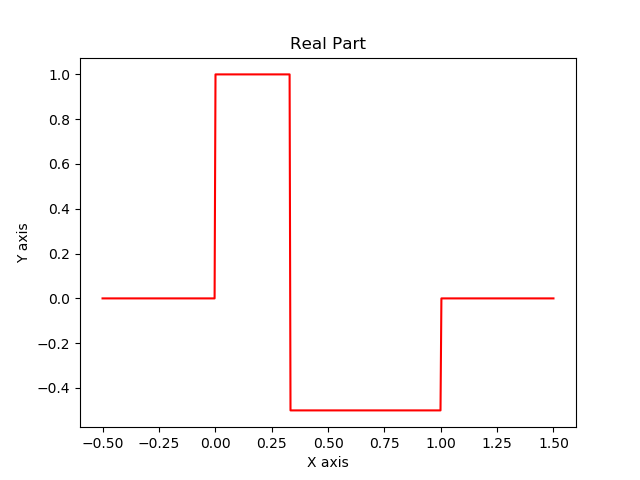
\includegraphics[width=\textwidth]{graphics/real_2.png}
    \caption{$\Real(\psi^{(3)}_2)$}
  \end{minipage}
  \hfill
  \begin{minipage}[b]{0.45\textwidth}
    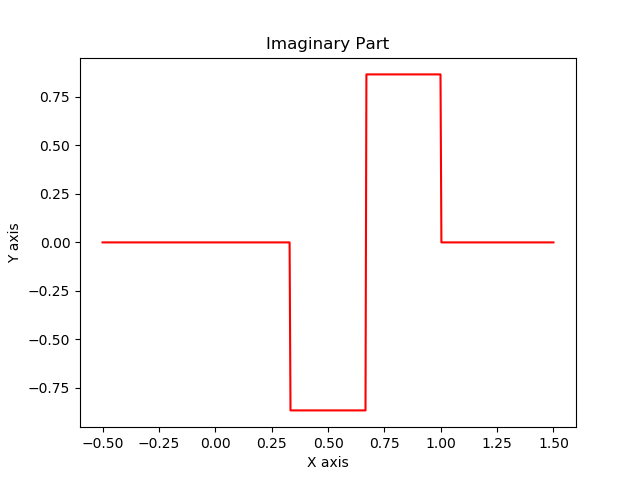
\includegraphics[width=\textwidth]{graphics/imag_2.png}
    \caption{$\Imag(\psi^{(3)}_2)$}
  \end{minipage}
\end{figure}
    
\end{frame}


\begin{frame}{The Monna map}

Every non-zero element $x \in \Qbb_p$ may be represented uniquely as a \txtblue{``Laurent series"} of the form
    \[x = \sum_{i = k}^{\infty} a_i p^i,\quad a_i = 0, ..., p-1, k \in \Zbb\]

\begin{block}{Definition:}
    Define $\rho: \Qbb_p \to \Rbb_+$ as follows
    \[\rho(\sum_{i = k}^{\infty} a_i p^i) = \sum_{i = k}^{\infty} a_i p^{-i - 1}\]
    This is called the \txtblue{Monna map} or a \txtblue{$p$-adic change of variables}.
    \vspace{\baselineskip}\\
    We define the \txtblue{pullback of $\rho$} as $\rho^*: L^2(\Rbb_+) \to L^2(\Qbb_p)$ where
    \[\rho^*(f) = f \circ \rho\]
\end{block}
    
\end{frame}


\begin{frame}{Kozyrev's Main Result}

\begin{block}{Theorem [Kozyrev, \cite{kozyrev_2002} and \cite{kozyrev_khrennikov_shelkovich_2014}]\footnote{The equalities here should be interpreted as an equality in $L^2$, as in it holds outside of a measure zero set}}

Let $W_j$ be given by the $p$-Haar wavelets,
\begin{itemize}
    \item $\{p^*(W_j)\}_{j \in \Zbb}$ forms an orthogonal decomposition of $L^2(\Qbb_p)$.
    \item The elements of this indicated basis are eigenvectors of the \txtblue{Vladimirov operator} defined as
    \[D^\alpha f(x) = \frac{p^\alpha - 1}{1 - p^{-1 - \alpha}} \int_{\Qbb_p} \frac{f(x) - f(y)}{|x - y|^{1+\alpha}_p} d\mu(y)\]
    such that
    \[\txtblue{D^\alpha} \rho^*(\psi_k^{(p)}(p^{-j} x - n)) = \txtblue{p^{\alpha(1 - j)}} \rho^*(\psi_k^{(p)}(p^{-j} x - n))\]
\end{itemize}
\end{block}
\end{frame}

\begin{frame}{Kozyrev Wavelets}

\begin{itemize}
    \item This connection illustrates a link between the theory of wavelets and $p$-adic spectral analysis.
    \item The collection $\{p^*(W_j)\}_{j \in \Zbb}$ is thus aptly called the \txtblue{$p$-adic wavelet basis} (or sometimes called the \txtblue{Kozyrev wavelet basis}).
\end{itemize}

This only marked the beginning of the theory of $p$-adic wavelets:
\begin{itemize}
    \item Generalizations to higher dimensions (ie. $\Qbb^d_p$) were later developed in \cite{khrennikov2006padic}.
    \item Methods of constructing other $p$-adic wavelets without using the Haar Wavelet were developed in \cite{khrennikov_shelkovich_2009} and \cite{khrennikov_shelkovich_2010}.
\end{itemize}
\end{frame}

\begin{frame}{Acknowledgements}
    The code used the generate the diagrams and my \txtblue{lecture notes} for this course can be found on:
    \begin{itemize}
        \item[{\includegraphics[scale=.75]{beamericonarticle}}] \url{https://github.com/maroon-scorch/APMA1940Y-notes}
    \end{itemize}
\end{frame}

\begin{frame}[allowframebreaks]
\frametitle{References}
% bibliography style is set to alpha here. you can experiment with other styles
\bibliographystyle{alpha}
% this line includes all references cited in the document. 
\bibliography{references.bib}
\end{frame}
\end{document}